\documentclass[letter,11pt]{article}

\usepackage{amsfonts}
\usepackage{amsmath}
\usepackage{amssymb}
\usepackage[brazilian]{babel}
\usepackage{enumerate}
\usepackage[T1]{fontenc}
%\usepackage[ansinew,latin1]{inputenc}
\usepackage[utf8x]{inputenc}
\usepackage{multicol}
\usepackage{graphicx}
\setlength\columnseprule{0.5pt}

\newtheorem{exer}{Exercício}
\newtheorem{teo}{Teorema}

\newcommand{\R}{\mathbb {R}}
\newcommand{\Z}{\mathbb {Z}}
\newcommand{\N}{\mathbb {N}}
\newcommand{\E}{\mathbb {E}}
\newcommand{\eqm}{\mbox{EQM}}
\newcommand{\sen}{{\rm \,sen}}
\newcommand{\V}{\mbox{Var}}

\newcommand{\var}{\mathrm{Var}}
\newcommand{\T}{\mathds{T}}
\newcommand{\sn}{\sum_{i=1}^n}
\newcommand{\hx}{\overline{X}}
\newcommand{\te}{\theta}
\renewcommand{\th}{\hat\theta}
\newcommand{\mn}{X_{(1)}}
\newcommand{\bs}{\boldsymbol}
\newcommand{\ix}{X_{(i)}}
\newcommand{\jx}{X_{(j)}}
\newcommand{\xx}{X_1X_2X_3X_4}

\newcommand{\mat}[1]{\mbox{\boldmath{$#1$}}}

\usepackage[letterpaper,top=3cm, bottom=2cm, left=2.5cm, right=2.5cm]{geometry}

\begin{document}

%\thispagestyle{empty}
\begin{center}{ \Large MAT02023 - Inferência A }\end{center}

\begin{center}
{\large  \sc Gabarito Lista 6 - Avaliação de Estimadores}
\end{center}
\vspace{15mm}


%%%%%%%%%%%%%%%%%%%%%%%%%%%%%%%%%%%%%%%%%%%%%%%%%%%%%%%%%%%%%%%%%%%%%%%%%%%%%%%
% Lista 8 Marcia

\begin{exer} \rm
%Explique com suas palavras o que é uma estatística suficiente.
\end{exer}



\begin{exer} \rm
%Explique com suas palavras o que é uma estatística suficiente mínima.
\end{exer}


% Questao Markus
\begin{exer} \rm
%Quais são as suposições do Teorema de Famílias Completas para a Família Exponencial. Comente as suposições.
\end{exer}


% Questao Markus
\begin{exer} \rm
%Fale sobre a suposição de suficiência no Teorema da Equivalência. Uma estatística pode ser minimal sem ser suficiente?
\end{exer}


% Questao Markus
\begin{exer} \rm
% Comente sobre as afirmações abaixo:  

\begin{enumerate}[a)]
  \item %Se existe uma estatística suficiente para $\theta$, então é minimal se for completa.

  \item %Uma estatística suficiente e completa é única.% função injetora (um a um) de uma estatística suficiente, suficiente minimal ou suficiente e completa é, respectivamente, ... .
\end{enumerate}

\end{exer}


\begin{exer}
\end{exer}
\includegraphics[scale=0.3]{gabarito_lista8_ex3_Marcia.jpg}




%%%%%%%%%%%%%%%%%%%%%%%%%%%%%%%%%%%%%%%%%%%%%%%%%%%%%%%%%%%%%%%%%%%%%%%%%%%%%%%
% Lista 2 Marcio

\begin{exer} \rm
\begin{enumerate}[a)]

\item Neste caso
\begin{equation}\label{e1}
\E(\hat\theta_1)=\te \quad \mbox{ e }\quad
\E(\hat\te_1)=\frac{2n\te+\sqrt n}{2(n+\sqrt n)}.
\end{equation}

\item Como $\E(\hat\te_1)=\te$, segue que
\[\eqm(\hat\te_1)=\var(\hat\te_1)=\frac{\te(1-\te)}{n}.\]
Para $\hat\te_2$, temos
\[\var(\hat\te_2)=\frac{1}{(n+\sqrt n )^2}\sum_{j=1}^n\var(X_j)=\frac{n\te(1-\te)}{(n+\sqrt n )^2}.\]
Com a ajuda de \eqref{e1}, podemos reescrever
$\mathrm{bias}(\th_2)^2$ como
\[\mathrm{bias}(\th_2)^2=\left[\frac{2n\te+\sqrt n}{2(n+\sqrt n)}-\te\right]^2=\frac{n(1-2\te)^2}{4(n+\sqrt n)^2},\]
de onde segue que
\[\eqm(\th_2)=\frac{n(1-2\te)^2}{4(n+\sqrt n)^2}+\frac{n\te(1-\te)}{(n+\sqrt n )^2}=\frac{n}{4(n+\sqrt n)^2}.\]
\end{enumerate}
\end{exer}


\begin{exer} \rm
\begin{enumerate}[a)]
\item Integrando por partes, obtem-se
$\E(X_j)=\te+1$, que implica $\E(\th_1)=\te+1$ (viciado). \item[]
Para $\th_2$, lembre que se $X_1,\cdots,X_n$ são variáveis
aleatórias contínuas, independentes e identicamente distribuídas
com função de distribuição $F$ e densidade $f$, então a densidade
de $X_{(1)}$ é dada por
    \[f_{X_{(1)}}(x)=n\big[1-F(x)\big]^{n-1}f(x).\]
    Neste caso temos $F(x)=1-e^{-(x-\te)}$, de onde segue que
    \[f_{X_{(1)}}(x)=ne^{-n(x-\te)}\quad\mbox{ e }\quad \E(\th_2)=\E(X_{(1)})=\te+\frac{1}{n}.\]
    Ou seja, $\th_2$ é viciado para todo $n\geq 1$ (mas é assintóticamente não-viciado).
\item Integrando por partes duas vezes, obtem-se
$\E(X_j^2)=\te^2+2\te+2$, de onde segue que
\[\eqm(\th_1)=\mathrm{bias}(\th_1)^2+\var(\th_1)=1+\E(\th_1^2)-\E(\th_1)^2=2.\]
Para $\th_2$, integrando-se por partes obtem-se, após alguma
álgebra
\[\E(X_{(1)}^2)=\left(\frac{1}{n}+\te\right)^2+\frac{1}{n^2},\quad\mbox{ e }\quad \var(X_{(1)})=\frac{1}{n^2}.\]
Disto segue que
\[\eqm(\th_2)=\frac{2}{n^2}\underset{n\rightarrow\infty}{\slongrightarrow}0.\]
Note também que $\eqm(\th_2)<\eqm(\th_1)$, para todo $n>1$.
\end{enumerate}
\end{exer}



\begin{exer} \rm
\begin{enumerate}
% \item[] 
% \item[(a)] Por simples integração obtem-se
% $E(\theta_1)=\E(X_i)=2\te/3$ (viciado). \item[] Para $\th_2$, lembre
% que se $X_1,\cdots,X_n$ são variáveis aleatórias contínuas,
% independentes e identicamente distribuídas com função de
% distribuição $F$ e densidade $f$, então a densidade de $X_{(n)}$ é
% dada por
%     \[f_{X_{(n)}}(x)=nF(x)^{n-1}f(x).\]
%     Neste caso,
%     \[f_{X_{(n)}}(x)=\frac{2nx^{2n-1}}{\te^{2n}}\quad\Longrightarrow \quad\E(\th_2)=\E(X_{(n)})=\frac{2n\te}{2n+1},\]
%     ou seja  $\th_2$ é viciado para todo $n\geq 1$ (mas é assintóticamente não-viciado). (Note que $\E(\th_1)>\E(\th_2), \forall n>1$).
% \item[(b)] Simples integração implica $\E(X_i^2)=\te^2/2$ de onde
% seque que
% \[\eqm(\th_1)=\frac{\te^2}{2}-\frac{4\te}{3}.\]
% \item[] Para $\th_2$, simples integração e alguma álgebra implica
% \[\E(X_{(n)}^2)=\frac{2n\te^2}{2n+1}\Longrightarrow\var(X_{(n)})=\frac{n\te^2}{(n+1)(2n+1)^2}\Longrightarrow\eqm(\th_2)=\frac{\te^2}{(n+1)(2n+1)}.\]
% Note que $(2n+1)(n+1)>2$ para todo $n\geq1$, assim (lembre que
% $\te>0$)
% \[EQM(\th_2)=\frac{\te}{(2n+1)(n+1)}<\frac{\te}{2}<\frac{\te}{2}-\frac{4\te}{3}=\eqm(\th_1),\]
% para todo $n\geq1$.
\end{enumerate}
\end{exer}


\begin{exer} \rm
\begin{enumerate}
% \item[] \item[(a)] Dica:
% \[X\sim N(0,\sigma^2)\quad\Longrightarrow\quad \frac{X_j}{\sigma}\sim N(0,1)\quad\Longrightarrow\quad \left(\frac{X_j}{\sigma}\right)^2\sim\chi_{(1)}^2.\]
% aplicando a dica segue que
% \[\E(\hat\sigma_c^2)=nc\sigma^2,\quad\var(\hat\sigma_c^2)=2nc^2\sigma^4, \quad EQM(\hat\sigma_c^2)=\underbrace{\big[(nc-1)^2+2nc^2\big]}_{:=Q(c)}\sigma^4.\]
% \item[(b)] Para minimizar $EQM(\hat\sigma_c^2)$, basta minimizar
% $Q(c)$ em $c$. O valor de $c$ tal que $Q(c)$ é mínimo é a solução
% da equação
% \[\frac{\partial Q(c)}{\partial c}=0\quad \Longrightarrow\quad c=\frac{1}{n+2}.\]
\end{enumerate}
\end{exer}


% ex10 Marcio lista 2
\begin{exer} \rm
\begin{enumerate}[a)]
\item $\E(\overline{X}) = \frac{\sum X_i}{n} = \frac{3\theta-2\theta^2+1}{4\theta+2}$.
Logo $\overline{X}$ é estimador viesado para $\theta$.

\item $\lim_{n \rightarrow \infty} \text{Viés}(\overline{X}) = \lim_{n \rightarrow \infty} \frac{\sum X_i}{n} = \lim_{n \rightarrow \infty} \frac{3\theta-2\theta^2+1}{4\theta+2} \diff \theta$.
Então $\overline{X}$ é assintoticamento viesado.

\item Como o estimador é assintóticamente viesado então não pode ser fortemente consistente.
\end{enumerate}


\noindent Obs.: Este exercício apresenta problemas pois $f_X$ será uma densidade
se, e somente se, $\theta=0$ ou $\theta=1$.
\end{exer}

% ex11
\begin{exer} \rm
Simples integração implica $\E(\overline{X})=\theta/(1+\theta)$.
\end{exer}

%
%%%%%%%%%%%%%%%%%%%%%%%%%%%%%%%%%%%%%%%%%%%%%%%%%%%%%%%%%%%%%%%%%%%%%%%%%%%%%%%%%%%%%
%\begin{exe} Seja $X_1,X_2,\cdots,X_n$ uma a.a., onde $X_j\sim U_c(0,1)$, para todo $j=1,\cdots,n$.  Encontre a distribuição da média geométrica
%$$Y_n=\left(\prod_{j=1}^{n}X_j\right)^{1/n}.$$ %Rohatgi pagina 307
%\end{exe}
%%%%%%%%%%%%%%%%%%%%%%%%%%%%%%%%%%%%%%%%%%%%%%%%%%%%%%%%%%%%%%%%%%%%%%%%%%%%%%%%%%%%%
%\begin{exe} Seja $X_1,X_2,\cdots,X_n$ uma a.a., onde $X_j\sim Exp(\lambda)$, para $j=1\cdots,n$.
%\begin{enumerate}[\bf(a)]
%\item Um estimador intuitivo para $\lambda$ é $\frac{1}{\overline{X}}$. Mostre que este é um estimador viciado para $\lambda$ e calcule o seu vício;
%\item Baseado no item {\bf (a)} encontre um estimador não viciado para $\lambda$;
%\end{enumerate}
%\end{exe}
%%%%%%%%%%%%%%%%%%%%%%%%%%%%%%%%%%%%%%%%%%%%%%%%%%%%%%%%%%%%%%%%%%%%%%%%%%%%%%%%%%%%%
%\begin{exe} Seja $X_1,X_2,\cdots,X_n$ uma a.a., onde $X_j$, para $j=1\cdots,n$, possui função densidade de probabilidade dada por $f_X(x)=e^{-(x-\theta)}$, para $\theta>0$ e $x>\theta$. Sejam $\overline{X}$ e $X_{(1)}$ dois estimadores para $\theta$. Encontre e compare os EQM's destes dois estimadores.
%\end{exe}
%%%%%%%%%%%%%%%%%%%%%%%%%%%%%%%%%%%%%%%%%%%%%%%%%%%%%%%%%%%%%%%%%%%%%%%%%%%%%%%%%%%%%
%\begin{exe} Seja $X_1,X_2,\cdots,X_n$ uma a.a., onde $X_j\sim U(0,\theta)$, para $j=1\cdots,n$. Mostre que $T(\mat{X})=\left(\prod_{j=1}^{n}X_j\right)^\frac{1}{n}$ é um estimador consistente para $\theta e^{-1}$.
%
%\noindent {\bf Dica:} Use $T^\ast(\mat{X})=\log(T(\mat{X}))$ e a Lei Fraca dos Grandes Números.%Rohatgi pagina 348
%\end{exe}
%%%%%%%%%%%%%%%%%%%%%%%%%%%%%%%%%%%%%%%%%%%%%%%%%%%%%%%%%%%%%%%%%%%%%%%%%%%%%%%%%%%%%
%\begin{exe} Seja $X_1,X_2,\cdots,X_n$ uma a.a., onde $X_j\sim U_c[0,\theta]$, para todo $j=1,\cdots,n$, $\theta \in \Theta=(0,\infty)$.  %Rohatgi pagina 348
%\begin{enumerate}[\bf(a)]
%\item Seja $M_n=\max(X_1,\cdots,X_n)$. Mostre que $M_n\longrightarrow^{\hspace{-.5cm}\prob}\hspace{.4cm}\theta$;
%
%\item Considere $Y_n=2\overline{X}$. Verifique se $Y_n$ é consistente para $\theta$.
%\end{enumerate}
%\end{exe}
%%%%%%%%%%%%%%%%%%%%%%%%%%%%%%%%%%%%%%%%%%%%%%%%%%%%%%%%%%%%%%%%%%%%%%%%%%%%%%%%%%%%%
%\begin{exe} Seja $X_1,X_2,\cdots,X_n$ uma a.a., onde $\E(X_j)=\mu$ e $\E|X_j|^2<\infty$, para todo $j=1,\cdots,n$. Mostre que
%
%$$T(\mat{X})=\frac{1}{2[n(n+1)]}\sum_{j=1}^{n}jX_j$$
%
%\noindent é um estimador consistente para $\mu$.
%\end{exe}
%%%%%%%%%%%%%%%%%%%%%%%%%%%%%%%%%%%%%%%%%%%%%%%%%%%%%%%%%%%%%%%%%%%%%%%%%%%%%%%%%%%%%
%\begin{exe} Seja $X_1,X_2,\cdots,X_n$ uma a.a., onde $\E(X_j)=\mu$ e $\V(X_j)=\sigma^2$, para todo $j=1,\cdots,n$, $\sigma^2$ finita. Verifique se  $\overline{X}$ and $S^2$ são estimadores consistentes de, respectivamente, $\mu$ e $\sigma^2$.
%
%\noindent {\bf Dica:} Seja $X_1,X_2,\cdots,X_n$ é uma a.a., onde cada $X_j$ possui função densidade de probabilidade $f_X(\cdot)$  e $\E|X_j|^p<\infty$, para algum inteiro positivo $p$ e $j=1,\cdots,n$. Então, para $1\leqslant k\leqslant p$,
% $$\frac{1}{n}\sum_{j=1}^{n}X_j^k\longrightarrow^{\hspace{-.5cm}\prob}\hspace{.4cm} \E(X^k).$$
%\end{exe}
%%%%%%%%%%%%%%%%%%%%%%%%%%%%%%%%%%%%%%%%%%%%%%%%%%%%%%%%%%%%%%%%%%%%%%%%%%%%%%%%%%%%%


% de onde?
\begin{exer} \rm 
% $X_1,X_2,\cdots,X_n$ uma amostra aleatória, onde $\E(X_j)=\mu$ e $\V(X_j)=\sigma^2$, para todo $j=1,\cdots,n$, $\sigma^2$ finita. Considere os estimadores para a média populacional
% 
% $$\widehat{\mu}_1=\overline{X}\quad\mbox{e}\quad \widehat{\mu}_2=\frac{X_1+X_n}{2}.$$
% 
% \begin{enumerate}[a)]
% \item Verifique se os estimadores são não viciados;
% 
% \item Qual dos estimadores é mais eficiente?
% 
% \item Analise os estimadores quanto à consistência.
% \end{enumerate}
\end{exer}
%%%%%%%%%%%%%%%%%%%%%%%%%%%%%%%%%%%%%%%%%%%%%%%%%%%%%%%%%%%%%%%%%%%%%%%%%%%%%%%%%%%%%
%\begin{exe} Seja $X_1,X_2,\cdots,X_n$ uma a.a., onde $X_j\sim Binomial(m_j,\rho)$, para todo $j=1,\cdots,n$, onde $m_j\geqslant1$ são constantes conhecidas. Seja
%
%$$T_1=\frac{\sum_{j=1}^{n}X_j}{\sum_{j=1}^{n}m_j}\quad\mbox{e}\quad T_2=\frac{1}{n}\sum_{j=1}^{n}\frac{X_j}{m_j}$$
%
%\noindent estimadores para $\rho$.
%
%\begin{enumerate}[\bf(a)]
%\item Encontre $\eqm(T_1)$;
%
%\item Encontre $\eqm(T_2)$;
%
%\item Qual dos estimadores é melhor?
%\end{enumerate}
%
%\noindent {\bf Dica:} Use $$\frac{1}{n}\sum_{j=1}^{n}m_j\geqslant\frac{n}{\sum_{j=1}^{n}\frac{1}{m_j}}.$$
%\end{exe}
%
%
%
%
%%%%%%%%%%%%%%%%%%%%%%%%%%%%%%%%%%%%%%%%%%%%%%%%%%%%%%%%%%%%%%%%%%%%%%%%%%%%%%%

\begin{exer} \rm
A prova do teorema pode ser vista em "Notas de Aula", página 64.
\end{exer}



\begin{exer} \rm
"Notas de Aula", página 65.
\end{exer}
    
    
\begin{exer} \rm
% Qual a diferença entre consistência forte e consistência fraca?
\end{exer}


\begin{exer} \rm
% Faça os seguintes exercícios do livro Statistical Inference: 
% \begin{enumerate}[a)]
% 	\item 7.9, 7.11 (a), 7.12 (b) e (c), 7.38, 7.40,  
% \end{enumerate}
\end{exer}
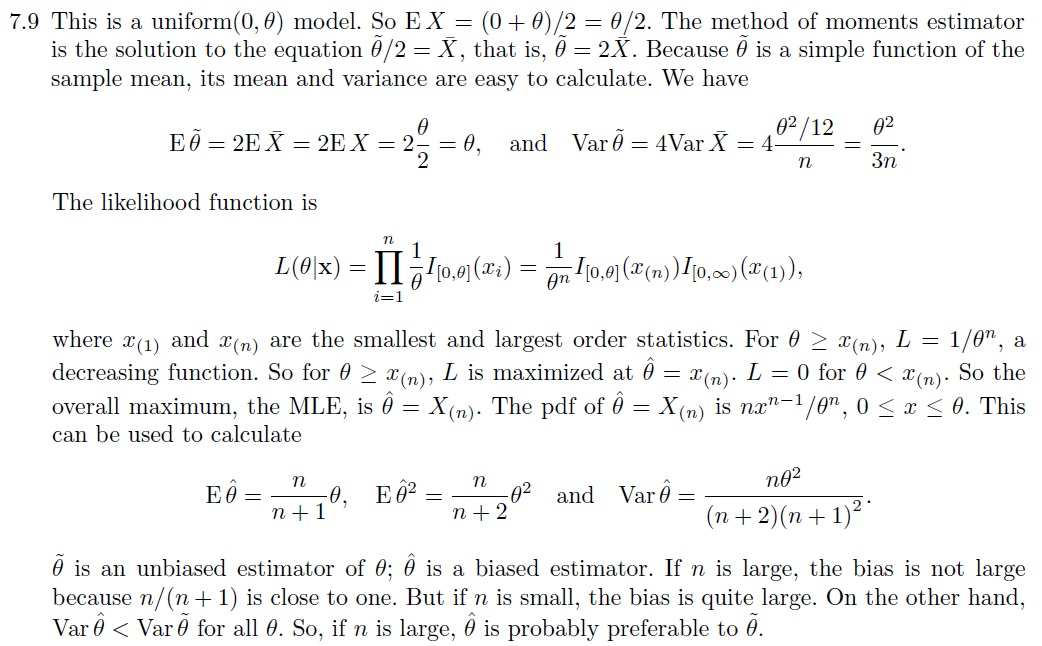
\includegraphics[scale=0.5]{gabarito_casella7_9.jpg}

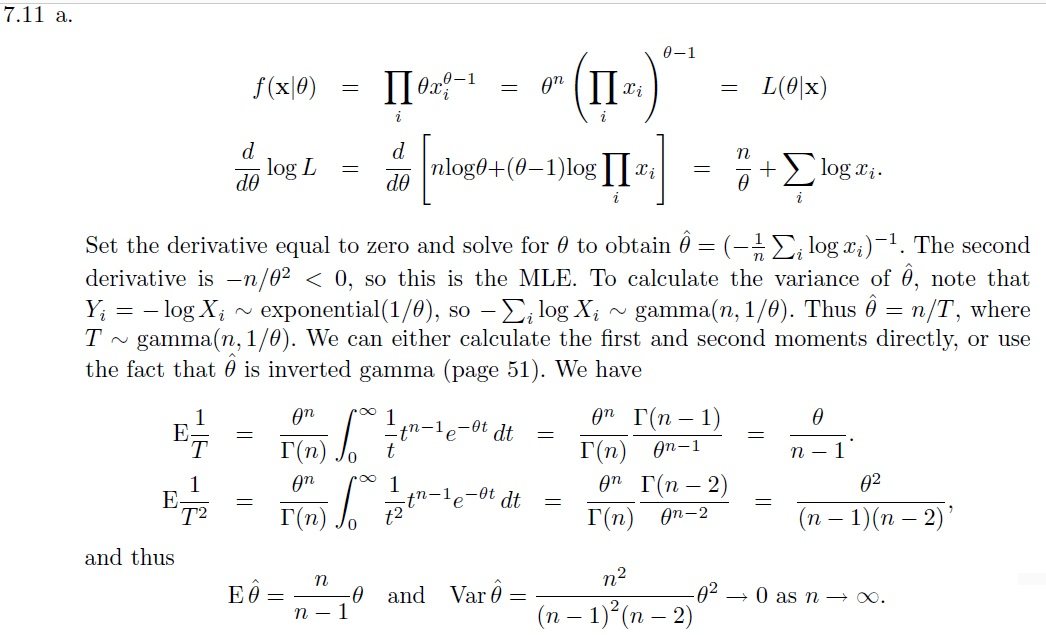
\includegraphics[scale=0.5]{gabarito_casella7_11a.jpg}

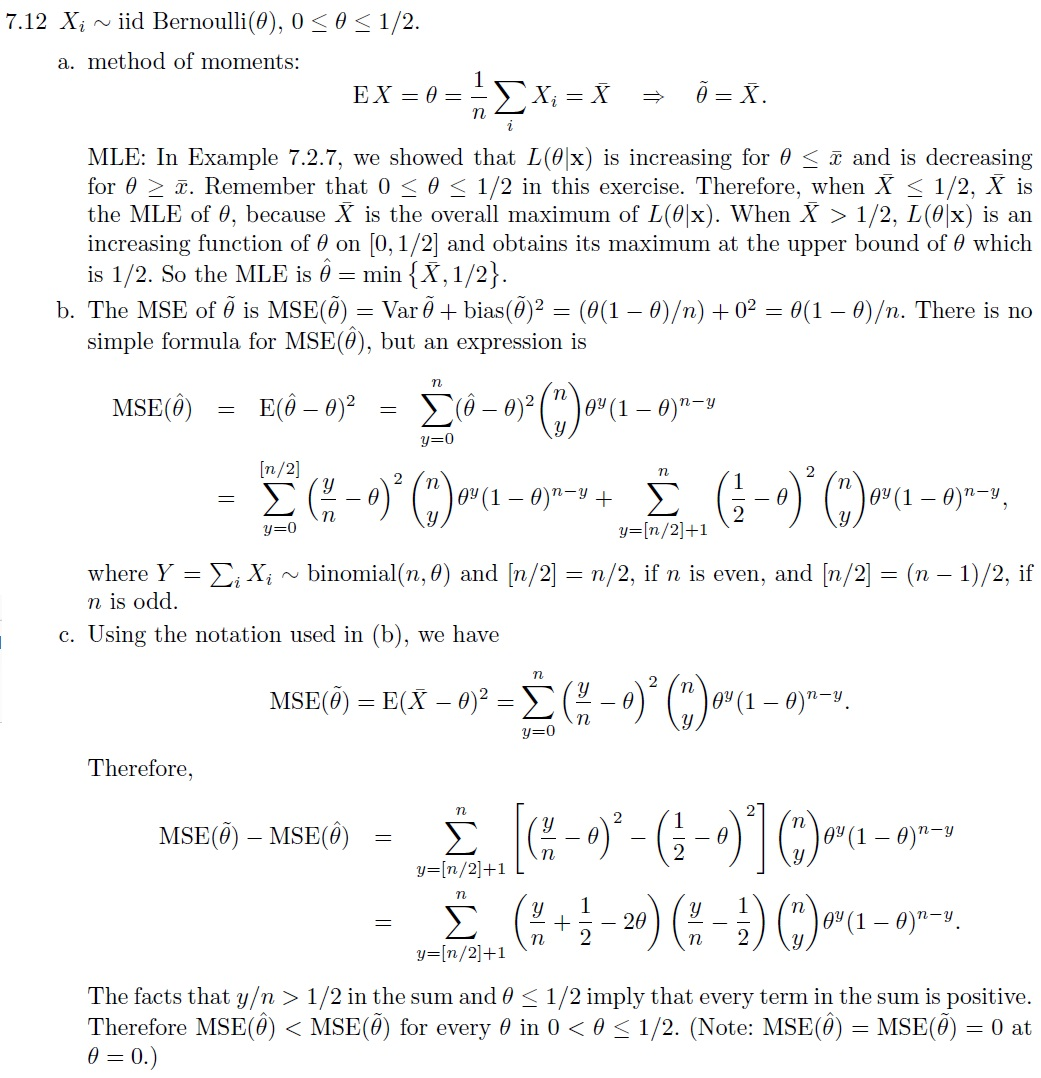
\includegraphics[scale=0.5]{gabarito_casella7_12.jpg}

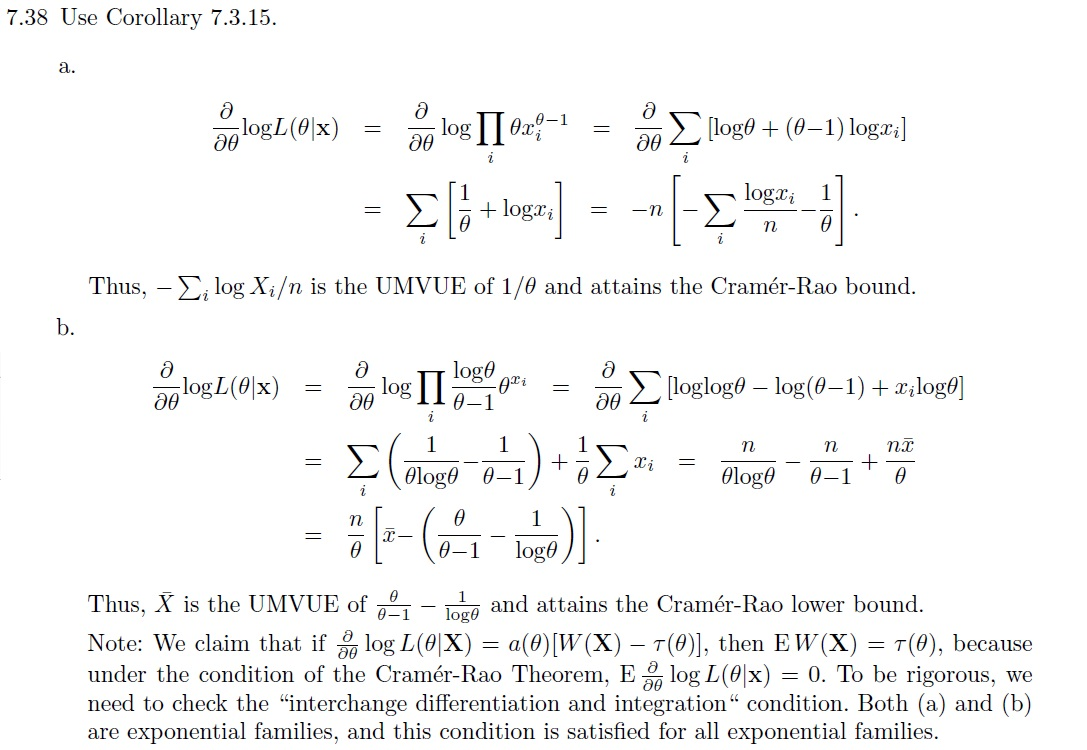
\includegraphics[scale=0.5]{gabarito_casella7_38.jpg}

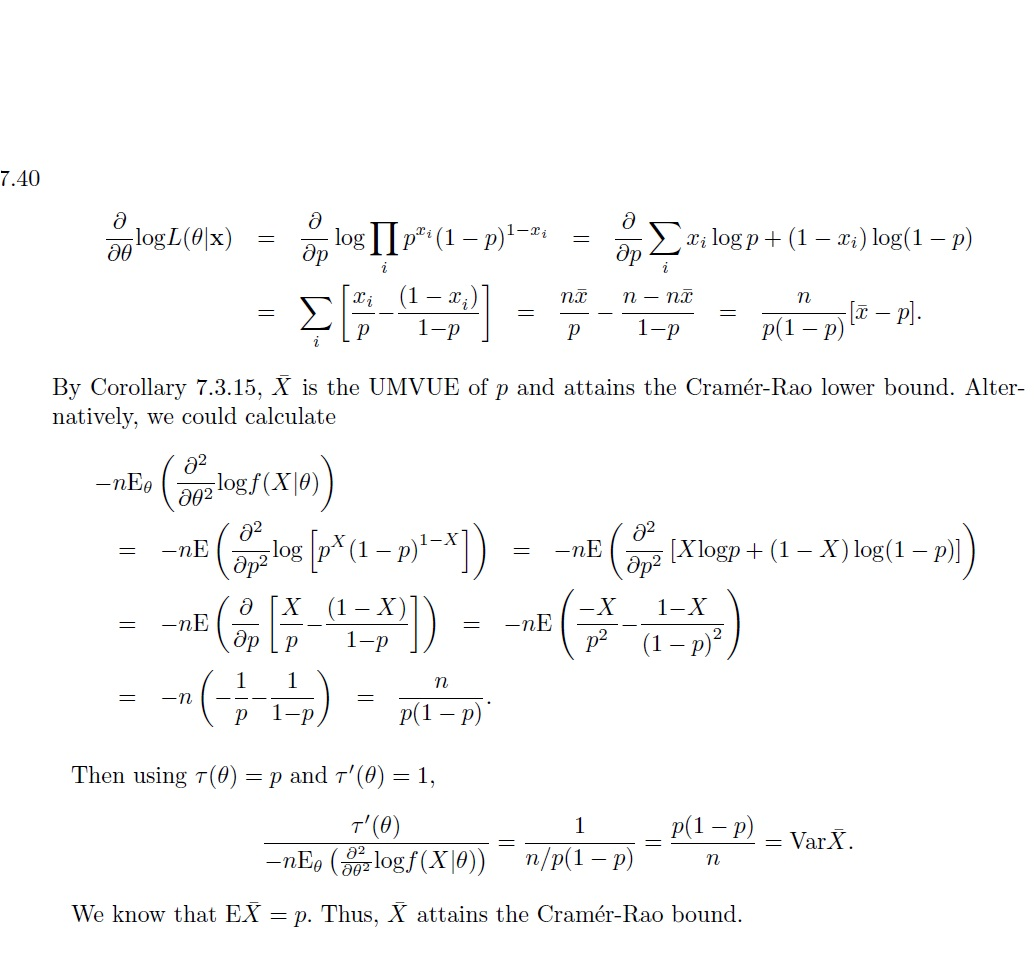
\includegraphics[scale=0.5]{gabarito_casella7_40.jpg}


\begin{exer} \rm
%lista %vinicius 1 
% Seja $X$ uma única observação da distribuição Bernoulli($\theta$). Considere os estimadores $T_1(X)=X$ e $T_2(X)=1/2$. %lista %vinicius 1
\begin{enumerate}[a)] 
\item %Os estimadores $T_1(X)$ e $T_2(X)$ são estimadores não-viciados para $\theta$?

\item %Calcule o EQM para $T_1(X)$ e $T_2(X)$.
\end{enumerate}

\end{exer}


\begin{exer} \rm
%lista %vinicius 9 
%Seja $X_1, \ldots, X_n$ uma amostra aleatória da densidade $f(x|\theta)=\theta(1+x)^{-(1+\theta)}I_{0, \infty}(x)$, em que $\theta > 0$.

\begin{enumerate}[a)] 

\item % Qual o estimador de máxima verossimilhança de $1/\theta$?

\item %Encontre o limite inferior de Cramér-Rao (LICR) para $e^{-\theta}$.
  LICR para $e^{-\theta}$ é $\frac{\theta^2e^{-2\theta}}{n}$.

\item %Encontre o LICR para a variância de um estimador não-viciado de $1/\theta.$
LICR para $\frac{1}{\theta}$ é  $\frac{1}{n\theta^2}$.

\end{enumerate}

\end{exer}





%%%%%%%%%%%%%%%%%%%%%%%%%%%%%%%%%%%%%%%%%%%%%%%%%%%%%%%%%%%%%%%%%%%%%%%%%%%%%%%
% lista 7 marcio
% \smallskip
% \begin{exer} \rm
% Seja $X_1,X_2,\cdots,X_n$ uma a.a. onde $X_j\sim N(\mu,\gamma_o^2\mu^2)$, para $j=1\cdots,n$, onde $\gamma_o^2>0$ é conhecido e $\mu>0$.
% \begin{enumerate}[a)]
%   \item Encontre uma estatística suficiente para $\mu$;
%   \item Mostre que $(\sum_{i=1}^{n}X_i,\sum_{i=1}^{n}X_i^2)$ é uma
% estatística suficiente e minimal;
%   \item Encontre $E[\sum_{i=1}^{n}X_i^2]$;
%   \item Encontre $E[(\sum_{i=1}^{n}X_i)^2]$;
%   \item Encontre
% \[E\left[\frac{n+\gamma_o^2}{1+\gamma_o^2}\sum_{i=1}^{n}X_i^2-\left(\sum_{i=1}^{n}X_i\right)^2\right].\]
% \end{enumerate}
% \end{exer}
% 
% %%%%%%%%%%%%%%%%%%%%%%%%%%%%%%%%%%%%%%%%%%%%%%%%%%%%%%%%%%%%%%%%%%%%%%%%%%%%%%%%%%%%
% \begin{exer} Seja $X_n$ uma amostra aleatória da densidade $f(x;\theta)=\theta(1+x)^{-(1+\theta)}I_{(0,+\infty)}(x). $
% \begin{enumerate}[\bf(a)]
% \item   Encontre o LICR para $e^{-\theta}$.
% 
% \item   Encontre o LICR para $1/\theta$.
% 
% \item   Encontre o LICR para $\theta^2+2$.
% \end{enumerate}
% 
% \end{exer}



% \vspace{0.5cm}
%%%%%%%%%%%%%%%%%%%%%%%%%%%%%%%%%%%%%%%%%%%%%%%%%%%%%%%%%%%%%%%%%%%%%%%%%%%%%%%%%%%%
\begin{exer} \rm
%Seja $X_1, \ldots, X_n$ uma amostra aleatória de uma $Exponencial(\lambda)$.
\begin{enumerate}[\bf(a)]
\item %Encontre, se possível, um estimador não viciado de variância uniformemente mínima (ENVVUM) para $1/\lambda$.
$\overline{X}$ é ENVVUM de $1/\lambda $.

\item %Encontre, se possível, um ENVVUM para  $\lambda$.
$\frac{(n-1)}{\sum_{i=1}^{n}X_i}$ é ENVVUM de $\lambda$.

\end{enumerate}
\end{exer}


% \vspace{0.5cm}
%%%%%%%%%%%%%%%%%%%%%%%%%%%%%%%%%%%%%%%%%%%%%%%%%%%%%%%%%%%%%%%%%%%%%%%%%%%%%%%%%%%%
\begin{exer} \rm
% Seja $X_1, \ldots, X_n$ uma amostra aleatória de uma $Binomial(k,p)$, com $k$ conhecido.
% Encontre, se possível, um ENVVUM para $P(X=1).$
$\frac{k\dbinom{k(n-1)}{\sum X_i -1}}{\dbinom{kn}{\sum_i X_i}}$
\end{exer}


% \vspace{0.5cm}
%%%%%%%%%%%%%%%%%%%%%%%%%%%%%%%%%%%%%%%%%%%%%%%%%%%%%%%%%%%%%%%%%%%%%%%%%%%%%%%%%%%%
\begin{exer} \rm 
% Suponha que quando o raio de um círculo é medido, é cometido um erro que tem uma distribuição $N(0,\sigma^2)$. Se forem realizadas $n$ medições independentes, encontre um estimador não viciado da área do círculo. É o melhor não viciado?
O modelo pode ser escrito como
\[X_i=r+\varepsilon_i,\quad\varepsilon_i\sim N(0,\sigma^2)\quad\Longrightarrow\quad X_i\sim N(r,\sigma^2).\]
Note que $\E(X_i)=r$ o que implica $\hat r=\hx$ é não viciado para $r$. Lembrando que a área de um círculo é dado por $A=2\pi r^2$, um argumento similar ao do exercício 2 mostra que $T(\bs X)=2\pi(\hx^2-\sigma^2/n)$ é não viciado para $A$. Além disso,
\[\var(T(X))=4\pi^2\var\left(\hx^2-\frac{\sigma^2}{n}\right)=4\pi^2\left(\frac{\sigma^4}{n^2}(3-\frac{1}{n^2})+r^2\frac{\sigma^2}{n}(6-\frac{2}{n})\right),\]
 $I(\te)=n/\sigma^2$ e $\mathrm{LICR}=16\pi^2r^2\sigma^2/n$. Note que $T(X)$ não é o melhor.
\end{exer}


% \vspace{0.5cm}
%%%%%%%%%%%%%%%%%%%%%%%%%%%%%%%%%%%%%%%%%%%%%%%%%%%%%%%%%%%%%%%%%%%%%%%%%%%%%%%%%%%%
\begin{exer} \rm 
% Seja $X_1,X_2,\cdots,X_n$ uma amostra aleatória, onde $X_1\sim Poisson(\lambda)$, e $\overline{X}$ e $S^2$ estimadores da média e da variância amostral.

  \begin{enumerate}[a)]
% \item Prove que $\overline{X}$ é o melhor estimador não viciado de $\lambda$.
% 
% \item Prove a identidade  $\E(S^2|\overline{X})=\overline{X}$ e utilize-a para demonstrar explicitamente que $Var(S^2)>Var(\overline{X})$.
\item Note que $\sn X_i$ é suficiente e completa para $\te$ e $\hx$ é não viciado para $\te$. Segue que $\th =\hx$ é UMVU pelo Teorema de Lehmann-Scheffé.
\item Note que
\[\E(S^2|\hx=t)=\frac{1}{n-1}\sn\E\big((X_i-t)^2|\hx=t\big)=\frac{1}{n-1}\sn\Big[\E(X_i^2|\hx=t)+t^2-2t\E(X_i|\hx=t)\Big].\]
Precisamos provar que o lado direito da igualdade é igual a $t$. Uma maneira de se provar isso é calculando
\[P\big(X_i=k|\hx=t\big)=\frac{P\big(\hx=t|X_i=k\big)P(X_i=k)}{P\big(\hx=t\big)}=\binom{k}{t}\left(\frac{1}{n}\right)^t\left(1-
\frac{1}{n}\right)^{k-t},\]

ou seja $X_i|\hx=t\sim \mathrm{Bin}(t,1/n)$, de onde o resultado segue. Para mostrar a desigualdade, note que
\[\E(S^2|\hx)=\hx\quad\Longrightarrow\quad\E(\hx)=\E(\E(S^2|\hx))=\E(S^2),\quad\Longrightarrow\quad \E(\hx^2)<\E\big([S^2]^2\big),\]
onde a última implicação segue da desigualdade de Jensen para esperanças condicionais (a desigualdade é estrita pois $x^2$ é uma função estritamente convexa).

  \end{enumerate}

\end{exer}


\end{document}
